\section{iOS}

\begin{breakbox}
\textbf{Interface Builder}: Now part
of Xcode, editor to create user interfaces and layouts

\textbf{iOS Simulator}: It is a simulator, not an emulator
\end{breakbox}

\subsection{View Controllers}

\begin{breakbox}
\boxtitle{Application Delegate}

\textit{@UIApplicationMain attribute creates entry point to your app and a
run loop that delivers input events to your app.}

\begin{lstlisting}[language=swift]
import UIKit
@UIApplicationMain
class AppDelegate: UIResponder, UIApplicationDelegate {
    ...
}
\end{lstlisting}
\end{breakbox}

\begin{breakbox}
\boxtitle{Storyboards}

\begin{itemize}
\tightlist
\item
  You can create your app's UI in the Main.storyboard file
\item
  Contains all of the app's view controllers and shows how they are
  connected to each other
\item
  You can zoom to a specific view controller to lay out its user
  interface
\end{itemize}

\end{breakbox}

\begin{breakbox}
\boxtitle{View Controller}

\begin{itemize}
\tightlist
\item
  Each view controller controls a view and its subviews
\item
  View controllers inherit from UIViewController
\item
  There are methods / hooks for when a view controller's view is loaded,
  appears, disappears, etc. $\Rightarrow$ View Controller Lifecycle
\item
  viewDidLoad(): The main view and its subviews are loaded from the
  Interface Builder file, but size \& position may not be set yet. This
  is a good method to perform additional setup (e.g., setting the text
  of a label, changing the background color of a view, adding additional
  subviews, \ldots{})
\end{itemize}
\end{breakbox}

\begin{breakbox}
\boxtitle{Tab Bar Controller}

\begin{itemize}
\tightlist
\item
  Displays a tab bar at the bottom that shows up to 5 tabs
\item
  The tab bar controller always shows the child view controller that is
  associated with the selected tab
\item
  Content of the tab bar is determined by the tabBarItem property of the
  individual view controllers
\end{itemize}
\end{breakbox}
\begin{breakbox}
\boxtitle{Navigation Controller}

\begin{itemize}
\tightlist
\item
  ``Manages a stack of view controllers to provide a drill-down
  interface for hierarchical content''
\item
  Sometimes also useful just to show a navigation bar with a title
\item
  Content of the navigation bar is determined by the current view
  controller's navigationItem property
\end{itemize}

\end{breakbox}

\begin{breakbox}
\boxtitle{Seques}

\begin{itemize}
\tightlist
\item
  View Controllers in the Storyboard are connected with segues
  (transitions)
\item
  Each segue has a kind (e.g., Show, Present Modally, etc.) and an
  identifier
\item
  During a segue, a new instance of the destination view controller
  class is created
\item
  Often, we need to pass data from the origin view controller to the new
  destination view controller

  \begin{enumerate}
  \def\labelenumi{\arabic{enumi}.}
  \tightlist
  \item
    Assign an identifier to each segue
  \item
    Override prepare(for:sender:) method in origin view controller
  \end{enumerate}
\end{itemize}

\begin{lstlisting}[language=swift]
class CurrentOrderViewController: UIViewController {
    // ...
    override func prepare(for segue: UIStoryboardSegue, sender: Any?) {
        if segue.identifier == "ShowAddBeverageViewController",
        let navController = segue.destination as? UINavigationController,
        let addBeverageViewController = navController.topViewController as? AddBeverageViewController {
            addBeverageViewController.apiClient = apiClient
            addBeverageViewController.coreDataStack = coreDataStack
        }
    }
    // ...
}
\end{lstlisting}
\end{breakbox}


\subsection{Views \& Auto Layout}

\begin{breakbox}
\begin{itemize}
\tightlist
\item
  Views are visible, rectangular regions on screen
\item
  Views draw content in their own rectangular area
\item
  Views can have multiple subviews and a single superview
\item
  Views receive touch events
\item
  View Coordinate System Origin is at top left corner
\item
  Each view has its own coordinate system
\item
  Views have a frame property of type CGRect (CG = Core Graphics)
\end{itemize}

\begin{lstlisting}[language=swift]
class ViewController: UIViewController {
    let redView = UIView()
    let greenView = UIView()
    override func viewDidLoad() {
        super.viewDidLoad()
        view.addSubview(redView)
        view.addSubview(greenView)
        
        let width = view.frame.size.width / 2
        let height: CGFloat = 100
        redView.backgroundColor = .red
        redView.frame = CGRect(x: 0, y: 20, width: width, height: height)
        greenView.backgroundColor = .green
        greenView.frame = CGRect(x: width, y: 20, width: width, height: height)
    }
}
\end{lstlisting}
\end{breakbox}

\begin{breakbox}
\boxtitle{Auto Layout}


\begin{itemize}
\tightlist
\item
  External changes (e.g., device rotates, different screen sizes, etc.)
\item
  Internal changes (e.g., content changes, app supports
  internationalization)
\item
  AutoLayout dynamically calculates the size and position of all the
  views in the view hierarchy, based on constraints placed on those
  views.
\item
  Layouts must be nonambiguous and satisfiable $\Rightarrow$ \textbf{there should be
  one and only one possible solution}

  \begin{itemize}
  \tightlist
  \item
    Ambiguous Layout: There is more than one solution.
  \item
    Unsatisfiable Layout: There is no solution.
  \end{itemize}
\end{itemize}

\end{breakbox}

\begin{breakbox}
\boxtitle{Constraints}

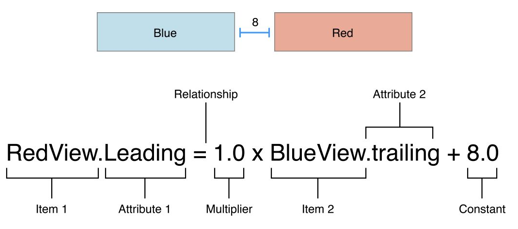
\includegraphics[width=.15\textwidth]{figures/constraint.png}

A constraint is a linear equation
\end{breakbox}

\begin{breakbox}
\boxtitle{Safe Area}

\begin{itemize}
\tightlist
\item
  The portion of your view that is unobscured by bars, home indicator,
  \ldots{}
\end{itemize}
\end{breakbox}

\begin{breakbox}
\boxtitle{Auto Layout in code}


\begin{lstlisting}[language=swift]
import UIKit
class ViewController: UIViewController {
    let redView = UIView()
    let greenView = UIView()
    override func viewDidLoad() {
        super.viewDidLoad()
        redView.backgroundColor = .red
//X= translatesAutoresizingMaskIntoConstraints
        redView.X = false
        greenView.backgroundColor = .green
        greenView.X = false
        setupLayout()
    }

    func setupLayout() {
        view.addSubview(redView)
        view.addSubview(greenView)
        let safeArea = view.safeAreaLayoutGuide
        redView.topAnchor.constraint(equalTo: safeArea.topAnchor).isActive = true
        redView.heightAnchor.constraint(equalToConstant: 100).isActive = true
        redView.leftAnchor.constraint(equalTo: safeArea.leftAnchor).isActive = true
        redView.widthAnchor.constraint(equalTo: safeArea.widthAnchor, multiplier: 0.5).isActive = true
        greenView.topAnchor.constraint(equalTo: safeArea.topAnchor).isActive = true
        greenView.heightAnchor.constraint(equalToConstant: 100).isActive = true
        greenView.leftAnchor.constraint(equalTo: redView.rightAnchor).isActive = true
        greenView.widthAnchor.constraint(equalTo: safeArea.widthAnchor, multiplier: 0.5).isActive = true
    }
}
\end{lstlisting}
\end{breakbox}

\begin{breakbox}
\boxtitle{Intrinsic Content Size}

\begin{itemize}
\tightlist
\item
  Some views don't require an explicit width or height constraint,
  because their content determines their default size.
\item
  These kinds of views have a so-called Intrinsic Content Size.
\end{itemize}
\end{breakbox}

\begin{breakbox}
\boxtitle{Content Hugging Priority}

\begin{itemize}
\tightlist
\item
  If you have two labels with no width constraint, which should grow
  first over the size of its content, when the superview grows?
\item
  The label with the highest content hugging priority want's to grow as
  late as possible, so first all other labels grow
\end{itemize}
\end{breakbox}

\begin{breakbox}
\boxtitle{Content Compression Resistance Priority}
\begin{itemize}
\tightlist
\item
  Which label should cut off its contents, when the superview shrinks?
\item
  The label with the higher horizontal content compression resistance
  priority wins, the other is cutted
\end{itemize}
\end{breakbox}

\subsection{Common Views \& Controls}

\begin{breakbox}
\begin{itemize}
\tightlist
\item
  Labels
\item
  Buttons
\end{itemize}

\begin{lstlisting}[language=swift]
override func viewDidLoad() {
    super.viewDidLoad()
    let button = UIButton(type: .custom)
    view.addSubview(button)
    button.setTitle("Do Something", for: .normal)
    button.addTarget(self, action: #selector(doSomething), for: .touchUpInside)
    
    let safeArea = view.safeAreaLayoutGuide
    button.translatesAutoresizingMaskIntoConstraints = false
    button.leftAnchor.constraint(equalTo: safeArea.leftAnchor).isActive = true
}
@objc func doSomething() { ... }
\end{lstlisting}

\begin{itemize}
\tightlist
\item
  The target is an object that implements the action method
\item
  The action is a selector (basically a glorified string) that describes
  the name / signature of that method
\end{itemize}
\end{breakbox}

\begin{breakbox}
\boxtitle{Outlets}
\begin{itemize}
\tightlist
\item
  When we add a label or some other subview in Interface Builder, we
  need a way to reference it.
\item
  Thus, we add a connection from Interface Builder to the corresponding
  view controller class (Control-Drag).
\item
  Outlet is an instance variable through which the view controller code
  can refer to the label / button / image view / \ldots{}
\end{itemize}
\end{breakbox}


\subsection{Table Views}

\begin{breakbox}
\boxtitle{UITableView}

\begin{itemize}
\tightlist
\item
  Displays a scrollable list of cells
\item
  Data is provided by a data source object $\Rightarrow$ has to adopt
  UITableViewDataSource
\item
  Cells are of type UITableViewCell
\item
  Cells are reused for efficiency reasons
\item
  There are predefined cell styles, but you can also create a custom
  UITableViewCell subclass.
\item
  The table view is divided into sections (by default there is one
  section)
\end{itemize}
\end{breakbox}